\documentclass[letter,10pt]{article}
\usepackage[letterpaper, margin=0.75in]{geometry}
\geometry{letterpaper}
\usepackage{graphicx}
\usepackage{bbding} % For checkmark in itemize
\newcommand*\tick{\item[\Checkmark]}
\newcommand*\fail{\item[\XSolidBrush]}
\usepackage{enumitem} % Resume enumerate
\begin{document}

\section{Multiple Choice}

\begin{enumerate}
    \item Which common Linux program can be used to identify the type for a given file?
    \begin{itemize}
        \tick file
        \fail type
        \fail uname
        \fail which
        \fail whoami
    \end{itemize}
    
    \item It's enough to look at the file extension to know what type of file it is.
    \begin{itemize}
        \tick False
        \fail True
    \end{itemize}
    
    \item Some file formats are executable, some are not. Besides PE32, which is another executable file format?
    \begin{itemize}
        \tick Mach-O
        \fail Fortran
        \fail Markdown
        \fail Common Document Format
    \end{itemize}
    
    \item Entry points apply to which file formats? (Select all that apply)
    \begin{itemize}
        \tick PE32
        \tick MACH-O
        \fail PDF
        \fail RTF
        \fail .DOCX
    \end{itemize}
    
    \item Which is NOT a feature or use case for a packer?
    \begin{itemize}
        \tick Improves operating system compatibility
        \fail Obfuscation
        \fail Smaller file size
        \fail Protects intellectual property
        \fail Thwart reverse engineering efforts
    \end{itemize}
    
    \item What is contained in the Rich Header?
    \begin{itemize}
        \tick Additional compiler/linker information
        \fail Name of the author
        \fail Number of sections
        \fail If the file is part of the operating system
    \end{itemize}
    
    \item After a good model is created, your job as a Data Scientist is complete.
    \begin{itemize}
        \tick False
        \fail True
    \end{itemize}
    
    \item If the \texttt{file} command doesn't specify a packer, does it mean the file is unpacked?
    \begin{itemize}
        \tick False
        \fail True
    \end{itemize}
    
    \item What might be the entropy level for an unpacked executable?
    \begin{itemize}
        \tick 5.5
        \fail 6.5
        \fail 7.5
        \fail 8.5
    \end{itemize}
    
    \item What might be the entropy level for a packed executable?
    \begin{itemize}
        \fail 5.5
        \fail 6.5
        \tick 7.5
        \fail 8.5
    \end{itemize}
    
    \item What is the most important area for consideration when making a model?
    \begin{itemize}
        \tick Ensuring the data is accurate and is a representative sample.
        \fail Using the Linux operating system.
        \fail Write code using Python.
        \fail Making use of GPU acceleration, or else training takes too long.
    \end{itemize}
    
    \item What might be a way to ensure the samples are diverse?
    \begin{itemize}
        \tick Use a similarity hash to make sure the files aren't alike.
        \tick Use AV Class to make sure there are a lot of different malware families in the dataset.
        \fail Make sure the SHA-1 or MD-5 hashes are different.
        \fail Take all the data available, and randomly select files from the collection for the dataset.
        \fail Trick question, this isn't an issue to consider.
    \end{itemize}
    
    \item Identify the algorithms which are similarity hashes (Select all that apply)
    \begin{itemize}
        \tick SSDeep
        \tick SDHash
        \tick LZJD
        \fail MD-5
        \fail SHA-1
        \fail RIPEMD
        \fail Whirlpool
    \end{itemize}
    
    \item Benign executables from \texttt{C:\textbackslash Windows} and \texttt{C:\textbackslash Program Files} provide enough variance to be the source for goodware samples for a malware vs. goodware model.
    \begin{itemize}
        \tick False
        \fail True
    \end{itemize}
    
    \item What technique can be used to have the model select the best features?
    \begin{itemize}
        \tick Regularization (ElasticNet)
        \fail Neural Networks
        \fail Low-entropy detection
        \fail False Positives
    \end{itemize}
    
    \item When would you use the \texttt{libsvm} file format for your dataset?
    \begin{itemize}
        \tick When the data is sparse
        \fail When analyzing PDF malware
        \fail When using entropy as a feature
        \fail When using the \texttt{pefile} Python module
    \end{itemize}
    
    \item A network monitoring tool, sometimes called ``hacking'' tools, shouldn't be considered malware for our purposes.
    \begin{itemize}
        \tick True
        \fail False
    \end{itemize}
    
    \item When the malware model gets a classification wrong for a given file, that sample could be:
    \begin{itemize}
        \tick Undiscovered malware
        \tick Weird or unusual goodware
        \fail Part of the training set
    \end{itemize}
    
    \item Shellcode:
    \begin{itemize}
        \tick Assembly code which does some action
        \tick Is the malicious payload for malware
        \fail Written in JavaScript
        \fail Works on any operating system
    \end{itemize}
    
    \item Which is NOT a type of malware (based on our definition)?
    \begin{itemize}
        \tick Plain text file
        \tick Hacking tools
        \fail Trojan
        \fail Fileless
        \fail Rootkit
        \fail Spyware
    \end{itemize}
    
    \item Malware gets on to a victim's computer by
    \begin{itemize}
        \tick Social Engineering
        \tick Software vulnerability
        \fail Magic
        %\fail Not using the computer % Misleading, malware can get on to an unattended computer.
        \fail Parallel port devices
    \end{itemize}
    
    \item Which is NOT a reason adversaries make malware?
    \begin{itemize}
        \tick Help the world
        \tick Keep vendors of security software employed
        \fail Steal information (espionage)
        \fail Break or damage infrastructure (sabotage)
        \fail Steal money
    \end{itemize}
    
    \item There's no such thing as Mac malware
    \begin{itemize}
        \tick False
        \fail True
    \end{itemize}
    
    \item Which is NOT a core concept of cybersecurity?
    \begin{itemize}
        \tick Accuracy
        \fail Integrity
        \fail Non-Repudiation
        \fail Confidentiality
        \fail Availability
    \end{itemize}
    
    \item Which is NOT a safety consideration for handling, storing malware?
    \begin{itemize}
        \tick Luck
        \tick Disconnecting the computer from the network
        \tick Use Windows XP
        \fail Use a different operating system
        \fail Encryption
        \fail Disallow execution on the partition or directory where the malware resides
        \fail Use a virtual machine
    \end{itemize}
    
    \item Some Windows or MS-DOS executable files but are NOT explicitly PE32 files include:
    \begin{itemize}
        \tick New Executable files
        \tick COM files
        \fail System drivers
        \fail Screen savers
    \end{itemize}
    
    \item Due to \textit{conceptual drift}...
    \begin{itemize}
        \tick A model which may have performed well will at some point begin to have degraded performance.
        \fail Malware gets more complex in nature.
        \fail People will stop using Windows.
        \fail Future models won't be trained with \texttt{libsvm} files.
    \end{itemize}
    
    \item What is NOT a use for Yara rules?
    \begin{itemize}
        \tick Determining the size of a malware sample.
        \fail Finding new samples of a given malware file.
        \fail Identifying malware samples by exploit or capability.
        \fail Sharing characteristics of malware samples with other researchers.
    \end{itemize}
    
    \item What is a use for $n$-grams?
    \begin{itemize}
        \tick Breaking down variable-sized data into a common length for all samples in the set.
        \tick Working with long linear data.
        \fail Working video files.
    \end{itemize}
    
    \item The presence of JavaScript in an Adobe PDF file is a clear indication of malware?
    \begin{itemize}
        \tick False
        \fail True
    \end{itemize}
    
    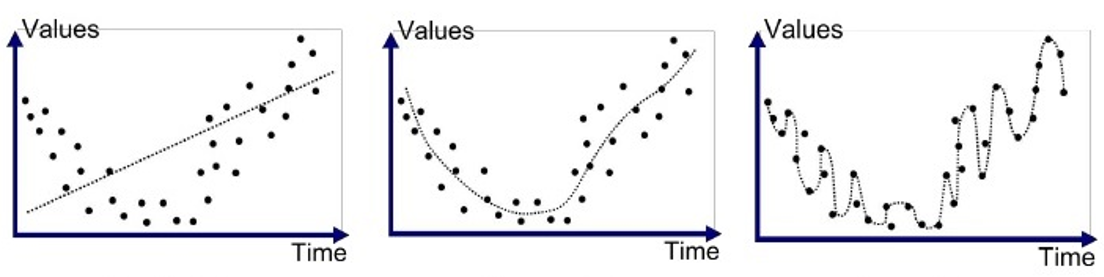
\includegraphics[scale=0.4]{../Images/fitting_sans_labels.png}
    \item Which graph shows the ideal situation when training a model?
    \begin{itemize}
        \fail First
        \tick Middle
        \fail Last
    \end{itemize}
    
    \item Besides simple accuracy, a model's performance might be measured by Recall, which is True Positives divided by True Positives + False Negatives, or Recall = TP/(TP+FN). Which is a reason for using Recall?
    \begin{itemize}
        \tick Making sure that all malware is caught, even if some goodware is called malicious.
        \fail Reducing goodware from being called malware.
        \fail Reducing errors in production.
    \end{itemize}
    
    \item Cross Validation is a technique which does what?
    \begin{itemize}
        \tick Breaks the data into parts, training a model in parts where each part of the data has been part of the test data.
        \fail A mechanism for feature selection to make the dataset smaller.
        \fail A way to evaluate multiple algorithms at once.
        \fail A procedure for changing an algorithm's parameters to find the best combination of parameters for a given dataset.
    \end{itemize}
    
\end{enumerate}
    
\newpage
\section{Free-Response or Essay Questions}
\begin{enumerate}[resume]
    \item Define malware.
    \begin{itemize}
        \tick Malicious \textit{intent} against computer \textit{owner}.
    \end{itemize}
    
    \item Define conceptual drift.
    \begin{itemize}
        \tick Over time, the malware changes, the malware authors change, so the features used, and the relationship between the features, will also change.
    \end{itemize}
    
    \item When would you want to use dynamic analysis over static analysis?
    \begin{itemize}
        \tick When the malware is packed and/or encrypted.
        \tick Malware is complete, it simply downloads another part which does further malicious behavior.
    \end{itemize}
    
    \item Why would it be acceptable to use AUC instead of accuracy as an acceptable metric for model performance?
    \begin{itemize}
        \tick A very high AUC means the accuracy was high too.
        \tick A high AUC shows that the model was able to accurate sort the files by malicious vs. benign.
    \end{itemize}
    
    \item For our purposes, why shouldn't a tool which might be used by a hacker, such as a port scanner, be considered malware?
    \begin{itemize}
        \tick We can't know the \textit{intent} of the user of the tool, and the author of the tool didn't \textit{intend} for malicious usage.
    \end{itemize}
    
    \item When might it be too difficult, or impossible, to create a Yara rule for a given malware family?
    \begin{itemize}
        \tick Malware family used different packers, or is otherwise not part of common source code.
        \tick Malware which is supposedly related, but having different characteristics, used for different things, but maybe attributed to a common attack, APT, or threat actor.
    \end{itemize}
    
\end{enumerate}

\end{document}